\documentclass[a4paper,12pt]{skthesis}
\usepackage{lgrind}
\usepackage{cmap}
%\usepackage[T2A]{fontenc}
\usepackage{lipsum}

% \newcommand{\gfcb}[1]{%
%     \fcolorbox{white}{gray!10!}{\quad\strut #1\quad}
%     } % gfcb := gray fcolorbox
% \newcommand{\cop}[1]{%
%     \texttt{\detokenize{#1}} 
%     } % cop := code output
\usepackage{csquotes} 
\usepackage{hyperref}
\usepackage{nameref}
\usepackage{amssymb}
\usepackage{xcolor}

\setcounter{secnumdepth}{1}

\begin{document}
% Everything with --rus inside is supposed to be written in russian

\title{Analyzing Transformer Language Models with Interpretative Techniques}
\titlerus{Анализ трансформерных языковых моделей с помощью интерпретационных методов}

\author{Pavel Shtykov}
\authorrus{Павел Штыков}

\department{Data Science}
\departmentrus{Науки о данных}

\degreemonth{June}
\degreeyear{2025}
\thesisdate{June 10}
\degreemonthrus{Июнь}
\thesisdaterus{Июнь 10}

\supervisorname{Serguei Barannikov}
% \supervisortitle{Assistant professor}
\supervisortitle{Leading research scientist}
% \supervisortitle{Associate professor}
\supervisordegree{PhD}

\supervisornamerus{Сергей Баранников}
% \supervisortitle{Assistant professor}
\supervisortitlerus{ведущий научный сотрудник}
% \supervisortitle{Associate professor}
\supervisordegreerus{к.м.н.}


% If you have cosupervisor, uncomment and fill these lines with name, title and degree of your cosupervisor
% Name and title fields are mandatory!
\cosupervisorname{Alexey Naumov}
\cosupervisortitle{Professor}
\cosupervisordegree{Doctor of Sciences}

\cosupervisornamerus{Алексей Наумов}
\cosupervisortitlerus{профессор}
\cosupervisordegreerus{д.ф.-м.н.}

% If you have two co-advisors uncomment the lines below
% \cocosupervisorname{Name2 Surname2}
% \cocosupervisortitle{Senior research scientist}
% \cocosupervisordegree{PhD}

% \cocosupervisornamerus{Имя Фамилия}
% \cocosupervisortitlerus{научный сотрудник}
% \cocosupervisordegreerus{д.ф.-м.н.}


\maketitle
\rusmaketitle

\setcounter{savepage}{\thepage}

\keywords{Transformer Language Models, Embedding Space, Model Interpretability, Hidden State Representation, Token Embeddings}
\begin{abstractpage}
This thesis explores a potential interpretative framework for transformer language models based on movement through embedding space. Current approaches often separate token embeddings from hidden states, potentially limiting understanding of these models.

The proposed framework considers hidden states as points within the embedding space, possibly forming a path from token to token. This perspective may offer an alternative view where each layer contributes to a trajectory culminating in next-token prediction.

Experiments with Llama models and custom-trained models suggest that weight-tied models show alignment between similarity metrics and model logits. Analysis indicates intermediate representations seem to diverge from the token embedding manifold in deeper layers. A regularization approach appears to constrain hidden states without significantly impacting performance.

These preliminary findings may support the framework's potential, though questions remain. The ability to train models with representation constraints without apparent performance degradation might suggest directions for more interpretable language models.

\end{abstractpage}

% \setcounter{page}{\thesavepage}
%  \begin{abstractpagerus}
%  \selectlanguage{russian}

%  \end{abstractpagerus}

%%%%%%%%%%%%%%%%%%%%%%%%%%%%%%%%%%%%%%%%%%%%%%%%%%%%%%%%%%%%%%%%%%%%%%
% -*-latex-*-
 % Your title pages, abstract
\tableofcontents
\newpage

% \listoffigures
% \newpage
% \listoftables

 % Probably you don't need to change it
\chapter{Introduction}

\paragraph{Relevance.}
Transformer-based language models have revolutionized natural language processing, yet our understanding of their internal representations remains limited. Current approaches often create an artificial separation between token embeddings and hidden states, hindering interpretability. As these models become increasingly integrated into critical systems, developing better interpretative frameworks is essential for ensuring reliability, enabling systematic debugging, and driving architectural innovations.

\paragraph{Main purpose of the research.}
This research aims to develop and validate a novel interpretative framework for transformer language models based on the concept of movement through embedding space. The central hypothesis posits that transformer operations can be understood as a trajectory from one token to the next, with each layer contributing to this path. Through analysis of pre-trained models and experiments with models trained under specific constraints, this work investigates whether this embedding space movement paradigm offers a valid perspective for understanding transformer behavior.

\paragraph{Scientific novelty.}
This thesis explores potential contributions to transformer interpretation: (1) a perspective that considers both token embeddings and hidden states as points within the same embedding space; (2) methods to examine this interpretative framework; (3) an experimental regularization approach that attempts to constrain intermediate hidden states within the token embedding manifold; and (4) preliminary evidence from both pre-trained models and models with alternative architectural configurations. While these contributions suggest possible directions for transformer interpretation, they represent initial steps that require further validation and refinement.

\paragraph{Statements for defense.}
The following statements are presented for defense:

1. The proposed interpretative framework of movement through embedding space offers a valid perspective for understanding transformer language models.

2. In standard pre-trained transformers, intermediate hidden states progressively diverge from the token embedding manifold as layer depth increases.

3. Intermediate hidden states can be constrained to remain within the vicinity of the token embedding cloud through regularization without significant performance degradation.

4. Different language modeling head architectures, including those explicitly based on similarity metrics, can achieve comparable performance.

\chapter{Author contribution}
% \chapter{List of publications}
% Below you can find examples how to cite your papers in this section (arxiv preprint, journal paper or part of the conference proceeding)

% \begin{enumerate}
%     \item Kingma D. P., Ba J. Adam: A method for stochastic optimization //arXiv preprint arXiv:1412.6980. --- 2014.
%     \item  Oseledets I. V. Tensor-train decomposition //SIAM Journal on Scientific Computing. – 2011. – Т. 33. – №. 5. – С. 2295-2317.
%     \item  Ulyanov D., Vedaldi A., Lempitsky V. Deep image prior //Proceedings of the IEEE conference on computer vision and pattern recognition. – 2018. – С. 9446-9454.
% \end{enumerate} % optional
\chapter{Literature review}

\section{Transformer Models and Interpretability}

Transformer-based language models have revolutionized natural language processing~\cite{vaswani2017attention}, yet they largely remain "black boxes" with limited interpretability. The field of transformer interpretability has grown significantly, with approaches like VisBERT by Aken et al.~\cite{aken2020visbert} providing visualization techniques for hidden states that offer insights into the model's internal processing.

\section{Geometric Interpretations of Transformer Representations}

A promising direction involves analyzing transformers through geometry in embedding space. Dar et al.~\cite{dar2022analyzing} present a framework where transformer parameters are interpreted by projecting them into embedding space, demonstrating that both pretrained and fine-tuned models can be understood through this lens.

Singh~\cite{singh2023analyzing} extends this by framing transformer dynamics as movement through embedding space, establishing a theory where intelligent behaviors map to paths in embedding space and context vectors are composed by aggregating token features. This aligns with our thesis's focus on interpreting transformers as inertial movement in embedding space.

The geometric properties of transformer hidden representations have also been explored by Valeriani et al.~\cite{valeriani2023geometry}, providing insights into information encoding across transformer layers.

\section{Alternative Formulations of Language Modeling}

Traditional transformers use a linear language modeling head, but alternative formulations enhance interpretability and performance. Geva et al.~\cite{geva2022transformer} showed that feed-forward networks in transformers function as key-value memories related to embedding space, suggesting a connection between internal representations and vocabulary token embeddings.

The relationship between k-nearest neighbors and transformer attention has been explored by Haris~\cite{haris2024knn}, who provides a theoretical framework for k-NN attention using Gaussian sampling for efficient approximation. Kernelized transformer variants have been investigated by Chowdhury et al.~\cite{chowdhury2021learning} and Simpson et al.~\cite{simpson2021kernel}, exploring Gaussian kernels and their integration with transformer architectures.

\section{Embedding Space Dynamics and Token Relationships}

The relationship between transformer hidden states and token embeddings has been studied from various angles. Song and Zhong~\cite{song2023uncovering} investigate hidden geometry in transformers by disentangling position and context. The concept of distances between hidden states and token embeddings, central to our research, has been touched upon by Aken et al.~\cite{aken2020visbert} and Dar et al.~\cite{dar2022analyzing}, providing a foundation for our investigation into the relationship between probability distributions and embedding distances.

\section{Research Gaps and Opportunities}

Despite advances in transformer interpretability, several key gaps remain:

Current approaches create an artificial separation between token embeddings and hidden states, hindering unified understanding of information flow through transformers. While geometric interpretations exist, the concept of viewing transformer operations as a continuous trajectory through embedding space remains underexplored.

The relationship between final hidden states and token embeddings has not been systematically investigated across different architectures, particularly regarding how proximity in embedding space correlates with token prediction probabilities in models with and without weight tying.

Additionally, methods to constrain intermediate hidden states within the token embedding manifold are lacking. These gaps present opportunities for developing a more intuitive framework for transformer interpretation by reconceptualizing operations as movement through embedding space.

\chapter{Problem statement}

\section{Notation and Preliminaries}

\subsection{Transformer Language Models}

We consider transformer-based language models as defined by \cite{vaswani2017attention}. Let $\mathcal{V}$ be a vocabulary of tokens, and let $\mathbf{E} \in \mathbb{R}^{|\mathcal{V}| \times d}$ be the embedding matrix, where $d$ is the embedding dimension. For a sequence of tokens $\mathbf{x} = (x_1, x_2, \ldots, x_n)$ with $x_i \in \mathcal{V}$, the transformer model processes the sequence through $L$ layers, producing hidden states $\mathbf{h}_i^l \in \mathbb{R}^d$ for each token $i$ at each layer $l$.

The final hidden state for token $i$ is denoted as $\mathbf{h}_i^L$. The language modeling head, typically a linear layer, transforms this hidden state into logits over the vocabulary:

\begin{equation}
    \mathbf{z}_i = \mathbf{W} \mathbf{h}_i^L + \mathbf{b}
    \label{eq::lm_head}
\end{equation}

where $\mathbf{W} \in \mathbb{R}^{|\mathcal{V}| \times d}$ and $\mathbf{b} \in \mathbb{R}^{|\mathcal{V}|}$ are the weight matrix and bias vector of the language modeling head, respectively. The probability distribution over the next token is then computed using the softmax function:

\begin{equation}
    P(x_{i+1} = v | x_1, \ldots, x_i) = \frac{\exp(z_{i,v})}{\sum_{v' \in \mathcal{V}} \exp(z_{i,v'})}
    \label{eq::softmax}
\end{equation}

\subsection{Embedding Space}

We define the embedding space as the $d$-dimensional vector space in which token embeddings and hidden states reside. For any token $v \in \mathcal{V}$, its embedding is denoted as $\mathbf{e}_v \in \mathbb{R}^d$, which corresponds to the $v$-th row of the embedding matrix $\mathbf{E}$.

The distance between two vectors $\mathbf{a}$ and $\mathbf{b}$ in the embedding space is measured using the Euclidean distance:

\begin{equation}
    d(\mathbf{a}, \mathbf{b}) = \|\mathbf{a} - \mathbf{b}\|_2 = \sqrt{\sum_{j=1}^d (a_j - b_j)^2}
    \label{eq::euclidean}
\end{equation}

\section{Research Problems}

This thesis addresses the following research problems:

\subsection{Relationship Between Probability Distributions and Embedding Distances}

We investigate the relationship between the probability distribution produced by the language modeling head and the distances between the final hidden state and token embeddings in the vocabulary. Specifically, we examine whether there exists a correlation between the probability assigned to a token and its proximity to the final hidden state in the embedding space.

For a given hidden state $\mathbf{h}$ and a token $v \in \mathcal{V}$, we study the relationship between $P(v|\mathbf{h})$ and $d(\mathbf{h}, \mathbf{e}_v)$, where $P(v|\mathbf{h})$ is the probability assigned to token $v$ by the language model given hidden state $\mathbf{h}$, and $d(\mathbf{h}, \mathbf{e}_v)$ is the Euclidean distance between $\mathbf{h}$ and the embedding of token $v$.

We hypothesize that there exists an inverse relationship between these quantities, such that tokens with higher probabilities tend to have smaller distances to the hidden state in the embedding space. To quantify this relationship, we use the Normalized Discounted Cumulative Gain (NDCG) metric:

\begin{equation}
    \text{NDCG} = \frac{\text{DCG}}{\text{IDCG}}
    \label{eq::ndcg}
\end{equation}

where DCG (Discounted Cumulative Gain) is computed based on the ranking of tokens according to their probabilities and inverse distances, and IDCG is the ideal DCG.

\subsection{Gaussian Kernel Language Modeling}

We propose an alternative formulation of the language modeling objective that replaces the traditional linear language modeling head with a learnable Gaussian kernel over k-nearest neighbors to token embeddings. The probability of the next token is computed as:

\begin{equation}
    P(x_{i+1} = v | x_1, \ldots, x_i) = \frac{\exp\left(-\frac{d(\mathbf{h}_i^L, \mathbf{e}_v)^2}{2\sigma_v^2}\right)}{\sum_{v' \in \mathcal{V}} \exp\left(-\frac{d(\mathbf{h}_i^L, \mathbf{e}_{v'})^2}{2\sigma_{v'}^2}\right)}
    \label{eq::gaussian_kernel}
\end{equation}

where $\sigma_v$ is a learnable parameter that controls the width of the Gaussian kernel for token $v$. This formulation makes the connection between hidden states and token embeddings more explicit and potentially more interpretable.

\subsection{Inertial Movement in Embedding Space}

TODO: This section will be filled in later with a description of the theoretical framework that interprets transformer operation as inertial movement in embedding space.

\section{Research Objectives}

Based on the research problems defined above, this thesis aims to:

\begin{enumerate}
    \item Empirically verify the relationship between probability distributions from the language modeling head and distances between hidden states and token embeddings in the vocabulary.
    
    \item Develop and evaluate a transformer model that uses a learnable Gaussian kernel over k-nearest neighbors to token embeddings instead of a traditional linear language modeling head.
    
    \item Formulate and validate a theoretical framework that interprets transformer operation as inertial movement in embedding space.
    
    \item Derive insights from these investigations that can guide the development of more interpretable and efficient transformer architectures.
\end{enumerate}

Through these objectives, we seek to contribute to a deeper understanding of how transformer language models process and represent information, with a particular focus on the geometric properties of their internal representations in embedding space.

\chapter{Methodology}

This chapter proposes an interpretative framework for transformer language models based on the concept of movement through embedding space.

The core insight is to view transformer operation as a trajectory from token $t_i$ to token $t_{i+1}$ in the embedding space. This process begins at the embedding of token $t_i$ and proceeds through a series of transformations as $L$ decoder layers are applied sequentially. Each decoder layer contributes an additive shift to the residual stream, creating a piecewise linear path through the embedding space, as illustrated in Figure \ref{fig:transformer_residual_sream}.

\begin{figure}[h]
    \centering
    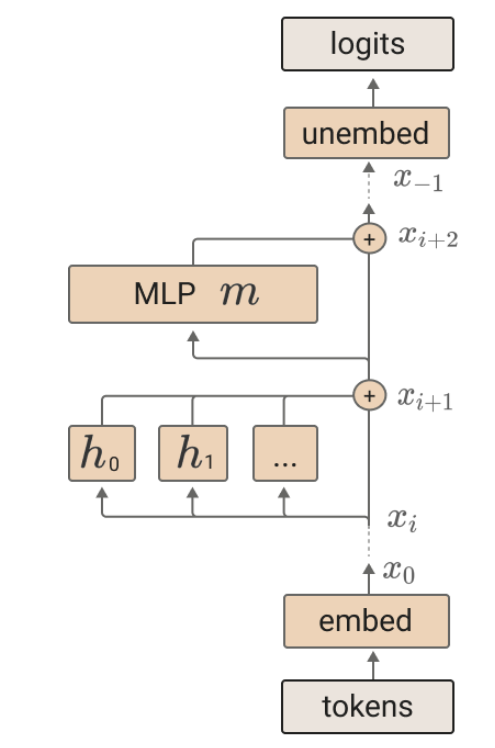
\includegraphics[height=0.5\textwidth]{images/residual_stream.png}
    \caption{Illustration of the decoder-only transformer operation from the residual flow perspective (adapted from \cite{math_framework_transformer}). In this illustration, intermediate hidden states are denoted as $x_0, x_1, \dots, x_{-1}$}
    \label{fig:transformer_residual_sream}
\end{figure}

After the final decoder layer produces the hidden state $\mathbf{h}_i^L$, the language modeling head generates a distribution over possible next tokens. The selection of token $t_{i+1}$ (via sampling or greedy selection) creates a "discontinuity" in the trajectory, as computation then continues from the embedding of this new token rather than from the final hidden state. Figure \ref{fig:my_transformer_schema} provides a simplified visualization of this token-to-token movement pattern.

\begin{figure}[h]
    \centering
    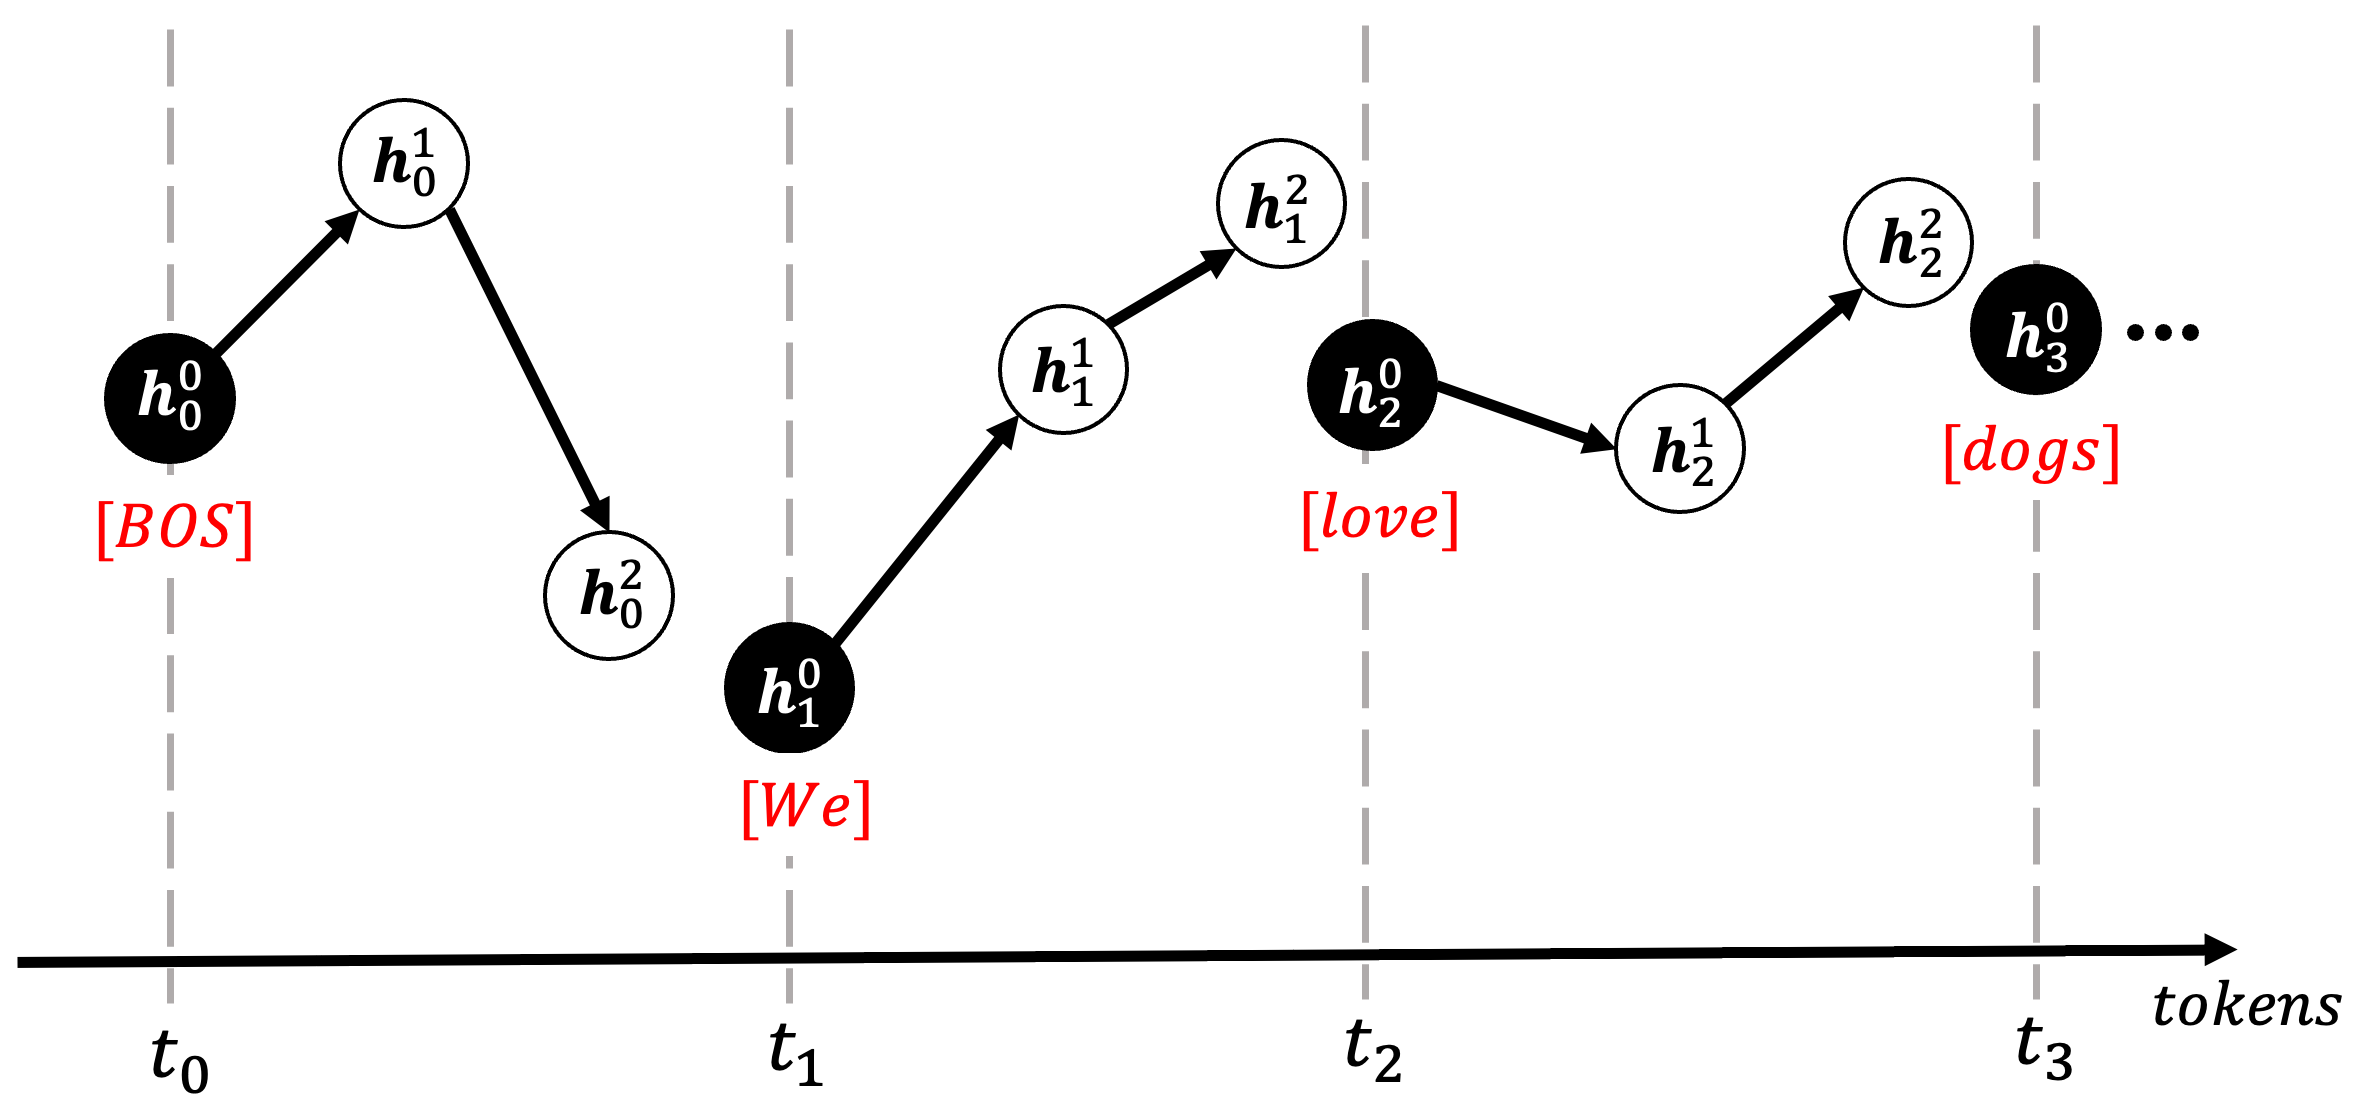
\includegraphics[width=0.75\textwidth]{images/my_transformer_schema_new.png}
    \caption{Simplified transformer operation diagram illustrating movement in embedding space. Filled circles represent token embeddings $t_{0}, t_{1}, \dots$, while empty circles represent intermediate hidden states $\mathbf{h}_0^0, \mathbf{h}_0^1, \mathbf{h}_1^0, \mathbf{h}_1^1, \dots$. The axis indicates the token sequence direction.}
    \label{fig:my_transformer_schema}
\end{figure}

To verify the applicability of the proposed interpretation to real transformers, the following analytical tools are suggested.

\section{Proximity Analysis Between Final Hidden States and Token Embeddings}\label{final_hidden_method}

A crucial aspect of the paradigm of movement in token embedding space is that the final hidden state should be close to the embedding of the next predicted token.

This behavior of the transformer can be visualized using the diagram in Figure \ref{fig:knn_schema}, which complements Figure \ref{fig:my_transformer_schema}.

\begin{figure}[h]
    \centering
    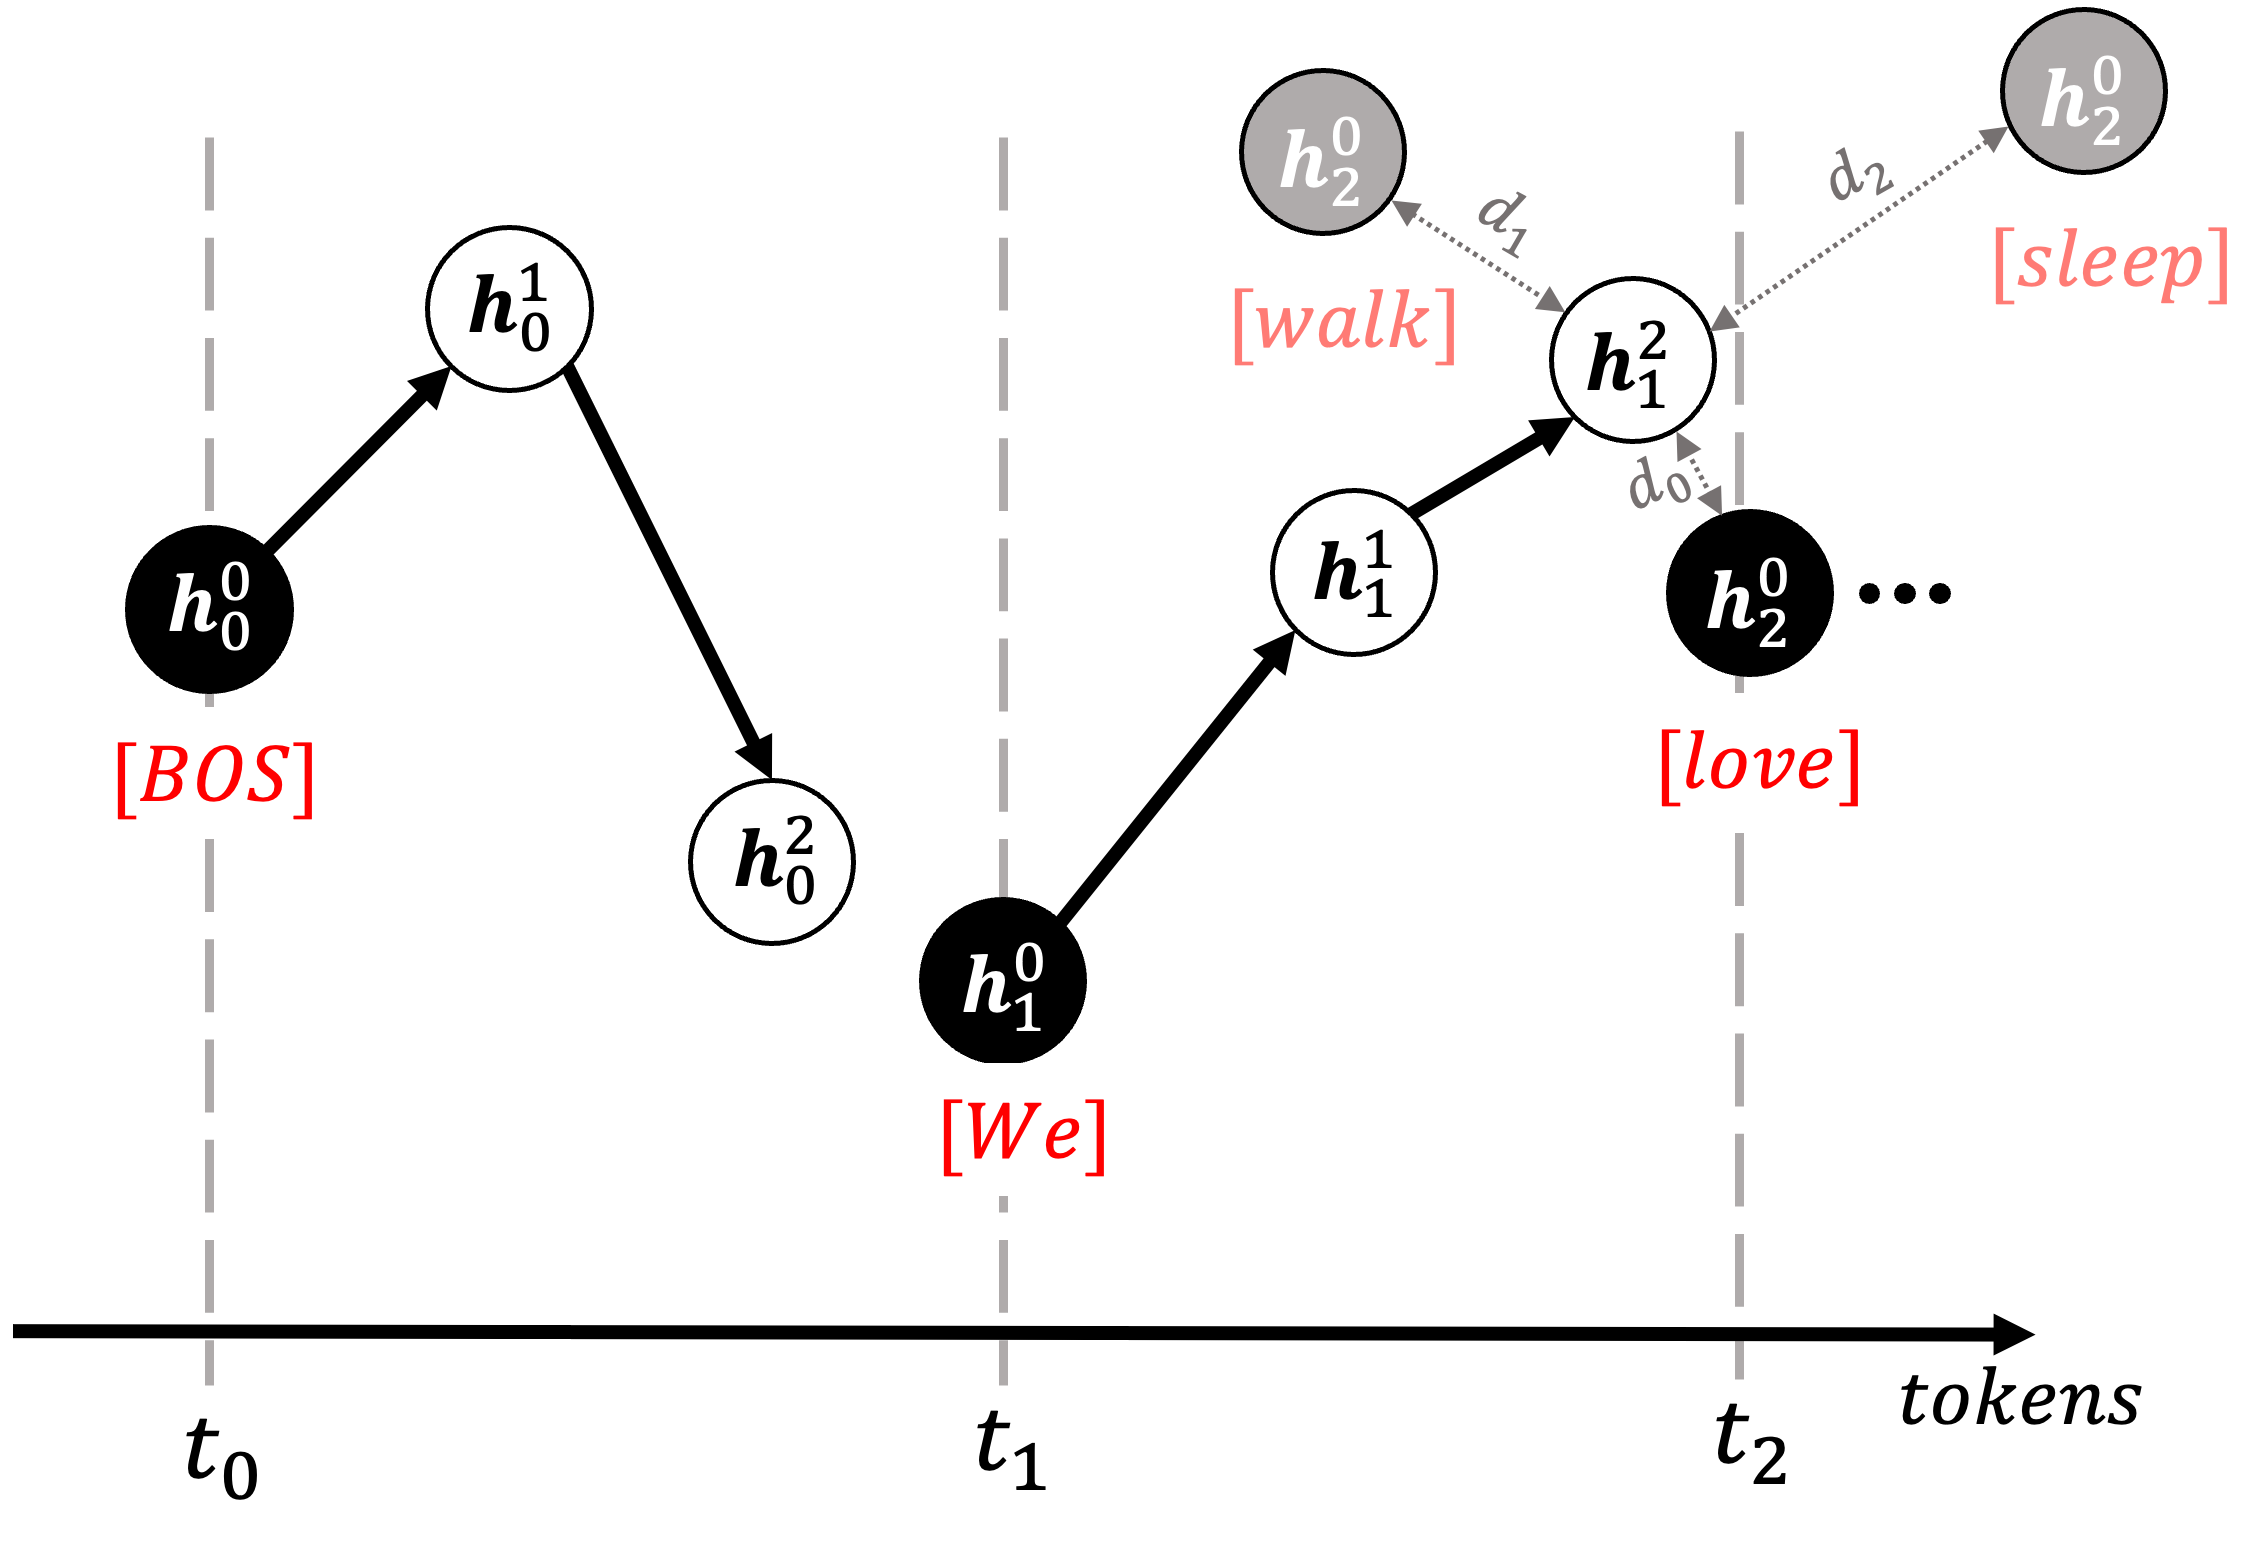
\includegraphics[width=0.6\textwidth]{images/knn_head_new.png}
    \caption{Illustration demonstrating the importance of proximity between the final hidden state $\mathbf{h}_i^L$ and the next token embedding $t_{i+1}$ in the proposed transformer interpretation paradigm. Distances is $d_j = \rho(h_1^2, t_j)$ and $d_0 < d_1 < d_2$.}
    \label{fig:knn_schema}
\end{figure}

To systematically evaluate this hypothesis, two complementary approaches are proposed: analyzing pre-trained transformers and training new models with specific constraints.

\subsection{Measuring Similarity Between Hidden States and Token Embeddings in Pre-trained Models}

To verify whether pre-trained transformers conform to this requirement, it is proposed to measure how well the distances between final hidden states and token embeddings correlate with the token probabilities predicted by the language modeling head for these same hidden states.

For this purpose, it is necessary to introduce a similarity metric between the final hidden state and all token embeddings in the model's vocabulary.

The first metric is Euclidean similarity. To measure this, the Euclidean distances are first calculated and then inverted by negation or taking the reciprocal:

\begin{equation}
d_{\text{Euclid}}(\mathbf{h}_i^L, \mathbf{e}_j) = \|\mathbf{h}_i^L - \mathbf{e}_j\|_2
\end{equation}

\begin{equation}
\text{sim}_{\text{NegEuclid}}(\mathbf{h}_i^L, \mathbf{e}_j) = -d_{\text{Euclid}}(\mathbf{h}_i^L, \mathbf{e}_j)
\end{equation}

\begin{equation}
\text{sim}_{\text{InvEuclid}}(\mathbf{h}_i^L, \mathbf{e}_j) = \frac{1}{d_{\text{Euclid}}(\mathbf{h}_i^L, \mathbf{e}_j)}
\end{equation}

Additionally, two other similarity metrics are considered: cosine similarity and dot similarity:

\begin{equation}
\text{sim}_{\text{cosine}}(\mathbf{h}_i^L, \mathbf{e}_j) = \frac{\mathbf{h}_i^L \cdot \mathbf{e}_j}{\|\mathbf{h}_i^L\|_2 \|\mathbf{e}_j\|_2}
\end{equation}

\begin{equation}
\text{sim}_{\text{dot}}(\mathbf{h}_i^L, \mathbf{e}_j) = \mathbf{h}_i^L \cdot \mathbf{e}_j = \sum_{k=1}^{d} h_{i,k}^L e_{j,k}
\end{equation}

To evaluate the alignment between model predictions and embedding space proximity, the correlation between language model logits and the similarity metrics is measured. This comparison employs the Normalized Discounted Cumulative Gain (NDCG), a standard metric for ranking quality assessment:

\begin{equation}
\text{NDCG@k} = \frac{\text{DCG@k}}{\text{IDCG@k}}
\end{equation}

where DCG@k (Discounted Cumulative Gain) is defined as:

\begin{equation}
\text{DCG@k} = \sum_{i=1}^{k} \frac{2^{\text{rel}_i} - 1}{\log_2(i+1)}
\end{equation}

Here, $\text{rel}_i$ is the relevance score of the item at position $i$, and IDCG@k is the DCG@k value for the ideal ranking. In this context, the relevance scores are derived from the token probabilities predicted by the language modeling head, and the comparison evaluates how well the similarity metrics align with these probabilities.

\subsection{Constructing Similarity-Based Language Modeling Heads for New Models}\label{scratch_final_hidden_info}

It is possible to attempt training a transformer with the desired properties from scratch. To do this, it is necessary to explicitly construct logits based on the proximity of the final hidden state to token embeddings.

For the case of dot similarity, such a construction method is well-known and is called weight tying. By tying the weight matrix in the language modeling head to the embedding matrix of the model, dot similarity is explicitly calculated as logits at the output of the language modeling head layer:

\begin{equation}
\text{LmHead}_{tied}(\mathbf{h}_i^L) = \mathbf{E} \mathbf{h}_i^L + \mathbf{b} = [\text{sim}_{\text{dot}}(\mathbf{h}_i^L, \mathbf{e}_1) + b_1, \ldots, \text{sim}_{\text{dot}}(\mathbf{h}_i^L, \mathbf{e}_{|\mathcal{V}|}) + b_{|\mathcal{V}|}]
\end{equation}

where $\mathbf{E} \in \mathbb{R}^{|\mathcal{V}| \times d}$ is the embedding matrix containing token embeddings $\mathbf{e}_j$, $\mathbf{h}_i^L \in \mathbb{R}^d$ is the final hidden state, and $\mathbf{b} \in \mathbb{R}^{|\mathcal{V}|}$ is the bias vector.

The Euclidean metric can also be approached in a similar manner. This involves simply outputting distances with a negative sign as logits at the layer output. Negation is chosen for simpler computation during training (inverting the distance is a more expensive operation). Such a layer is termed KnnHead:

\begin{equation}
\text{KnnHead}(\mathbf{h}_i)_j = \text{sim}_{\text{NegEuclid}}(\mathbf{h}_i^L, \mathbf{e}_j) + b_j = -\|\mathbf{h}_i^L - \mathbf{e}_j\|_2^2 + b_j
\end{equation}

Note that the squared Euclidean distance is used for computational efficiency, as it preserves the same ordering of distances while avoiding the square root operation.

Cosine similarity is not utilized as a head function when training transformers from scratch in this framework.

\section{Analyzing Intermediate Hidden States in Embedding Space}\label{reg_info}

Beyond the proximity of the final hidden state to the next token, the position of all intermediate hidden states is also crucial in this interpretative framework. It is logical to expect that intermediate hidden states should reside somewhere in the vicinity of the vocabulary token embeddings, since the transformer's movement in this paradigm occurs specifically from token to token.

For studying the position of intermediate hidden states in pre-trained transformers, the simplest approach is to examine their norms and visualize how these norms change depending on the layer number or the token position in the sentence. Heatmap visualizations of these norm patterns will be presented in the numerical experiments section.


When training a transformer from scratch, it is possible to explicitly penalize the model when certain intermediate hidden states deviate too far from the cloud of token embedding points. This can be implemented through a regularizer that linearly penalizes those intermediate hidden states whose norm exceeds the mean norm of token embeddings plus one and half standard deviations:

\begin{align}
    \mathcal{R}(\mathbf{h}_i^l) &= \lambda \cdot \max(0, \|\mathbf{h}_i^l\|_2 - (\mu_{\mathbf{E}} + \frac{3}{2} \sigma_{\mathbf{E}})) \\
    \mu_{\mathbf{E}} &= \frac{1}{|\mathcal{V}|}\sum_{j=1}^{|\mathcal{V}|}\|\mathbf{e}_j\|_2 \\ 
    \sigma_{\mathbf{E}} &= \sqrt{\frac{1}{|\mathcal{V}|}\sum_{j=1}^{|\mathcal{V}|}(\|\mathbf{e}_j\|_2 - \mu_{\mathbf{E}})^2}
\end{align}

where $\mathcal{R}(\mathbf{h}_i^l)$ is the regularization penalty for hidden state $\mathbf{h}_i^l$, $\lambda$ is the regularization coefficient, and $\|\mathbf{h}_i^l\|_2$ is the L2 norm of the hidden state. The total regularization term would be the average of penalties across all hidden states and tokens:

\begin{equation}
\mathcal{R}_{\text{total}} = \frac{1}{n \cdot L} \cdot \sum_{i=1}^{n} \sum_{l=1}^{L} \mathcal{R}(\mathbf{h}_i^l)
\end{equation}

This regularization encourages intermediate hidden states to remain within a reasonable distance from the token embedding cloud, reinforcing the concept of movement through embedding space.

\chapter{Numerical experiments}

In this section the results of numerical experiments should be placed.
They can confirm or contradict the expectation from the previous sections. 
The forms of result presentation are plots, tables, histograms, pictures, etc.
\begin{enumerate}
    \item Enumerating languages and programs used in the research.
    \item Describing in detail data sets you used.
    \item Presenting the metrics used.
    \item Presenting the results achieved in the experiment.
    \item Comparing the results of the experiment with those obtained using other methods.
    \item Outlining the benefits of the used method.
\end{enumerate}

\begin{table}[!htb]
    \centering
     \caption{
     The description of the table. Highlighting the main point following from this table.}
    \begin{tabular}{cccc}
    \toprule
         & Method 1 & Method 2 & Method 3  \\
        \midrule
      Metric 1   & $\mathbf{10}$ & $20$  & $30$ \\
      Metric 2   & $0.9$ & $0.4$ & $\mathbf{0.1}$ \\
      \bottomrule
    \end{tabular}
    \label{tab::methods_metrics}
\end{table}

Main requirements to plots:
\begin{itemize}
    \item sufficiently large font size for legend, axis labels, axis ticks;
    \item proper scale of y-axis: linear or logarithmic;
    \item clear difference in the rendering of lines corresponding to different methods.
\end{itemize}
\begin{figure}[!htb]
    \centering
    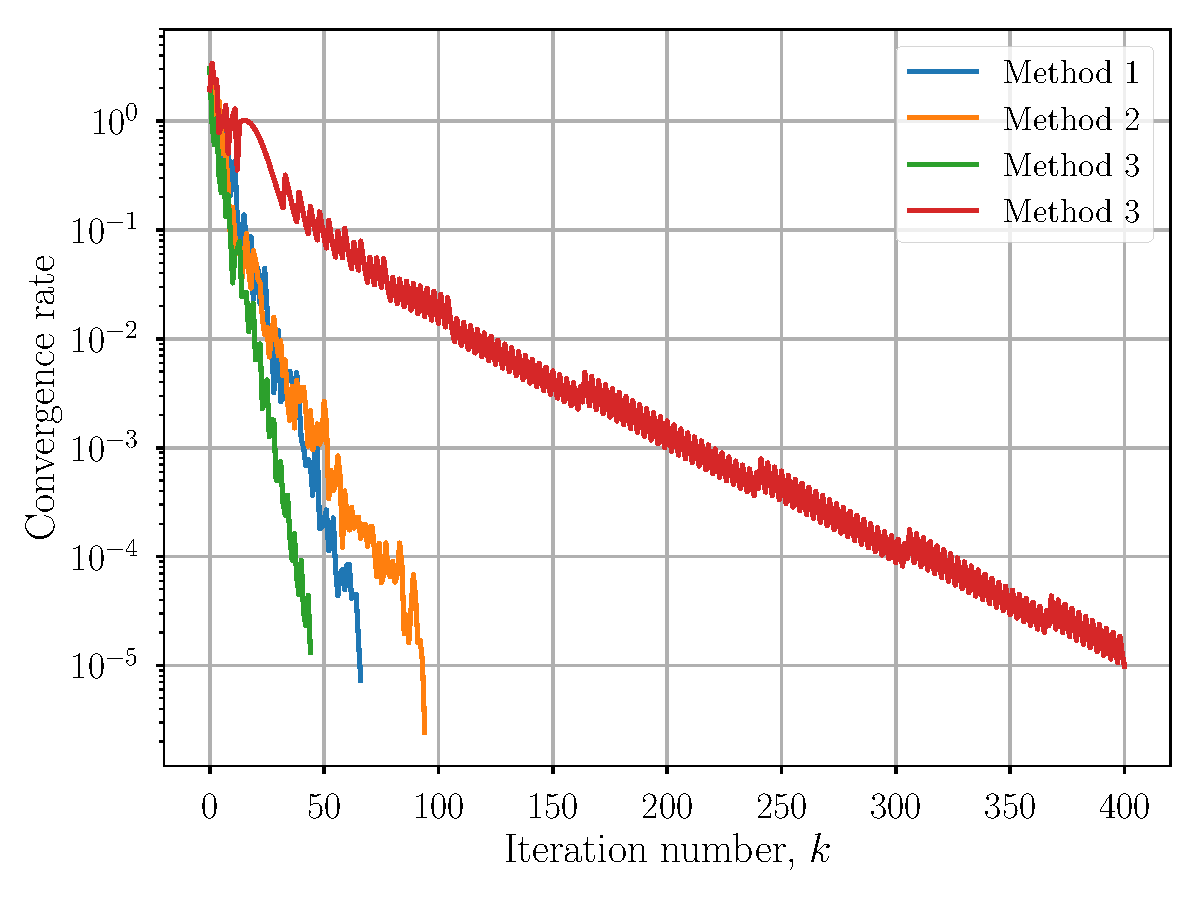
\includegraphics[width=0.4\textwidth]{images/test_plot.pdf}
    \caption{Comparison of the considered methods}
    \label{fig::x_vs_y}
\end{figure}



\chapter{Discussion and conclusion}
% Add details about content
    Summarize your work in this section.
    \begin{enumerate}
        \item Summary of the main results of the work that is consistent with the Aim and Objectives.
        \item Overall position on the global research landscape.
        \item Comparative critical analysis: what you have deduced from the findings and how these results relate to previous research or other studies.
        \item Research limitations.
    \end{enumerate}
    
\newpage
\chapter*{Acknowledgements}
\addcontentsline{toc}{chapter}{Acknowledgements}
    Write here acknowledgments of financial assistance for the conduct of research and to specific individuals who contributed to the science. 
    Dedications are not recommended and must reference scientific contributions.
\chapter*{Innovations}
\addcontentsline{toc}{chapter}{Innovations}

Innovation component of your research project (if any), i.e.:
        \begin{itemize}
            \item Start-up potential 
            \item Industrial application of research results
        \end{itemize} % optional
\addcontentsline{toc}{chapter}{Bibliography}
\bibliographystyle{acm}
\bibliography{Bibliography}
\chapter*{Appendix}
\addcontentsline{toc}{chapter}{Appendix} % optional
\end{document}

